\section{Introduction}
Small language models running on local hardware are useful when they can answer more questions correctly with a manageable inference budget. For graph reasoning, the model must track node identities and combine edges across the supplied input. Long identifiers consume tokens without changing the graph operation. Additional reasoning may help, but its preparation also costs resources. We therefore study a practical sequence: simplify the complete input representation, then test whether a short earlier trace improves the answer enough to justify its additional model-token use.

Our starting point is Zou and Tang's Trace as State: earlier reasoning is fed back before an unchanged source, with the same trace placed afterward as a matched control \citep{tang2026trace}. This study first reproduces that intervention on locally served small models and then develops a bounded compact-input adaptation. Related work improves reasoning through intermediate steps, repeated reading and additional inference-time computation \citep{wei2022cot,xu2024rereading,snell2025testtime}. Prompt compression reduces input length through content selection \citep{jiang2023llmlingua,pan2024llmlingua2}. These approaches motivate input-side and reasoning-side interventions, but their results do not establish which combination is useful under our local small-model configurations. Our initial five-trace reproduction encountered context, decoding and answer-interface boundaries and did not establish the original placement advantage.

We adapt that intervention by combining reversible node recoding with one short source pass. A deterministic dictionary replaces long identifiers throughout the complete source, examples and question, without removing edges or using gold answers. The small model first reads this compact input with a short output cap; its full thinking field is then supplied to a fresh reader. Direct compact reading isolates the added value of the trace package, while a byte-identical appended trace tests placement. An inverse dictionary restores predicted node identities. The evaluated recipe requires no model training, and charges each reused answer the entire preparation pass.

An independently frozen confirmation on twenty-four previously unused graphs shows that a front trace raises Qwen3-1.7B mean F1 from 0.6542 to 0.7703, at 39.8\% more preparation-inclusive model tokens than compact direct reading. In prespecified secondary comparisons, compact direct reading improves F1 over original input while using 42.4\% fewer model tokens; these comparisons are unadjusted for multiplicity. Front-versus-back superiority remains uncertain, and a separate practical 8K-capacity criterion fails despite compact-input fit. These findings support a bounded choice between lower-token compact reading and a more accurate trace package, rather than a universal cost-saving claim.

Our main contributions are:
\begin{itemize}
\item A local reproduction of the five-trace intervention, with explicit context, output-budget and answer-interface boundaries.
\item An independently confirmed small-model graph recipe that combines complete reversible inputs with one short trace, separating representation gains from the added trace-package benefit.
\item Audited preparation-inclusive accounting and complete reporting of failed criteria and uncertain comparisons, enabling the observed accuracy--token trade-off to be assessed without assuming latency or monetary savings.
\end{itemize}

\section{Related Work}
\label{sec:related-work}
\subsection{Reasoning traces, rereading and inference-time computation}
Chain-of-thought prompting uses intermediate reasoning demonstrations to improve reasoning in the evaluated sufficiently large models \citep{wei2022cot}. Self-consistency samples multiple reasoning paths and aggregates their answers \citep{wang2023selfconsistency}; Re2 repeats the question within a prompt to improve input understanding \citep{xu2024rereading}. Snell et al. study verifier search and sequential revisions, finding that effective compute allocation depends on problem difficulty \citep{snell2025testtime}. These results motivate careful budget allocation, but do not guarantee that more reasoning is beneficial for every small model. Our adaptation reuses one native thinking field without voting, a learned verifier or reader retraining. Reader repeats estimate variability; they are not an answer ensemble.

Trace as State is the direct methodological antecedent. Zou and Tang serialize earlier traces before the source on a fresh pass and compare against the same traces after the source \citep{tang2026trace}. We reproduce that placement intervention locally, then explicitly change its trace count and input representation in the compact extension. The confirmed prefix-versus-compact result tests the whole added trace package, including its warning wrapper; it neither isolates placement as the cause nor establishes the original theoretical memory separation in our models.

\subsection{Prompt compression and complete input representations}
LLMLingua combines a budget controller, iterative token-level compression and distribution alignment to shorten prompts \citep{jiang2023llmlingua}. LLMLingua-2 distills compression data and learns an extractive token classifier with bidirectional context \citep{pan2024llmlingua2}. Both address natural-language prompt compression. Our narrower transformation exploits arbitrary graph identifiers: a bijective dictionary shortens their representation while retaining the complete graph and operation. Inverse substitution restores the original prompt exactly. This is a task-specific representation control, not a general semantic summarizer or a new compression architecture. We have not run a head-to-head comparison with these compressors, and claim no superiority over them.

\subsection{Effective context use and structured evaluation}
Lost in the Middle shows that models can be sensitive to where relevant information appears in long inputs \citep{liu2024lost}. RULER distinguishes nominal context size from usable performance through retrieval, multi-hop tracing, aggregation and question answering \citep{hsieh2024ruler}. These studies support separating input feasibility from successful task completion. We use OpenAI GraphWalks parent and BFS tasks \citep{openai2025graphwalks}, whose answers can be independently recomputed, and locally served Qwen variants \citep{yang2025qwen3,qwen2026qwen35card}. Our contribution is an audited small-model replication and bounded adaptation on this structured benchmark, with complete preparation costs and failure reporting. It does not establish transfer to natural documents, improvements over direct CPU graph algorithms, or cross-question trace reuse.

\section{Methods}
\label{sec:migration-contract}

Figure~\ref{fig:method-pipeline} summarizes the complete compact-input pipeline. Figure~\ref{fig:method-overview} shows the preserved graph structure, and Figure~\ref{fig:method-modules} details its reversible representation and accounting boundary.
\begin{figure}[htbp]
\centering
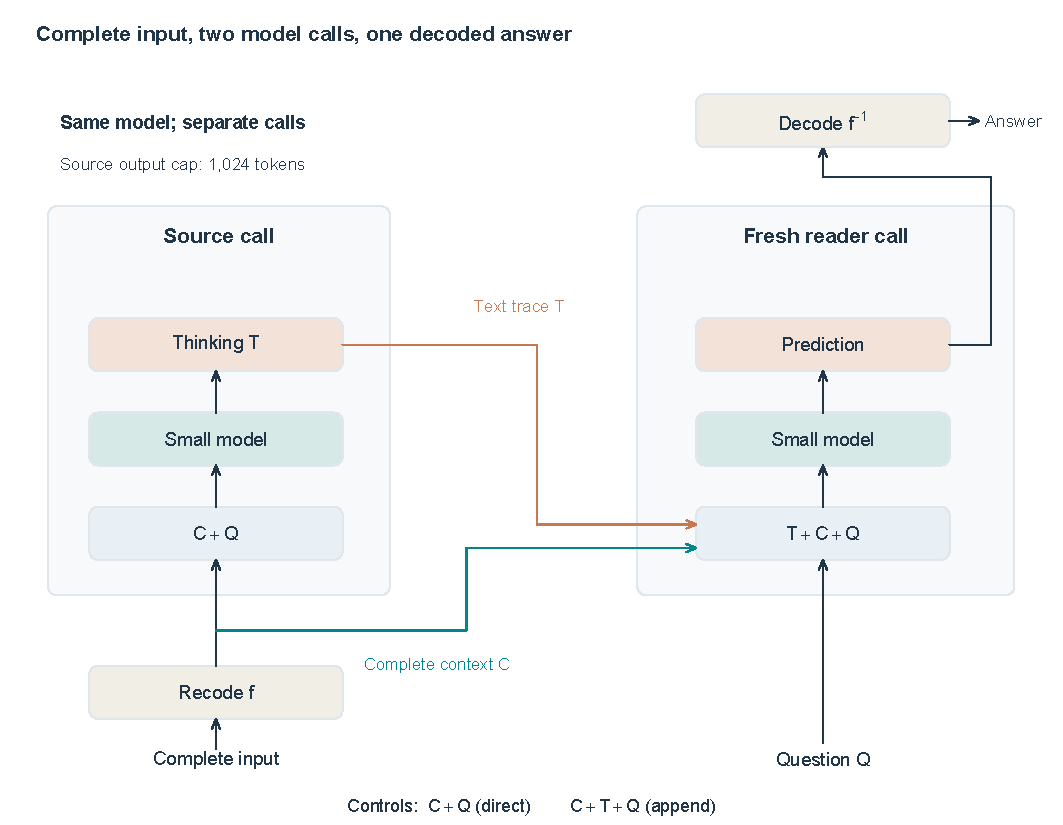
\includegraphics[width=.92\linewidth]{figures/polished_three_20261015/pipeline/publication.pdf}
\caption{Overall compact-input and single-trace method. The shaded groups are separate calls to the same small model. Reversible recoding $f$ produces the complete compact context $C$. The source reads $C+Q$ and supplies its native thinking $T$ to a fresh reader; the complete context also reaches that reader intact. Prefix assembles $T+C+Q$, and the stored inverse dictionary restores original identifiers afterward. The same operation $Q$ is used in both calls. Only text is transferred, not hidden states; the separate source answer is excluded. Direct and append controls use the indicated orders. Every trace answer includes the full source-call cost.}
\label{fig:method-pipeline}
\end{figure}
\begin{figure}[htbp]
\centering
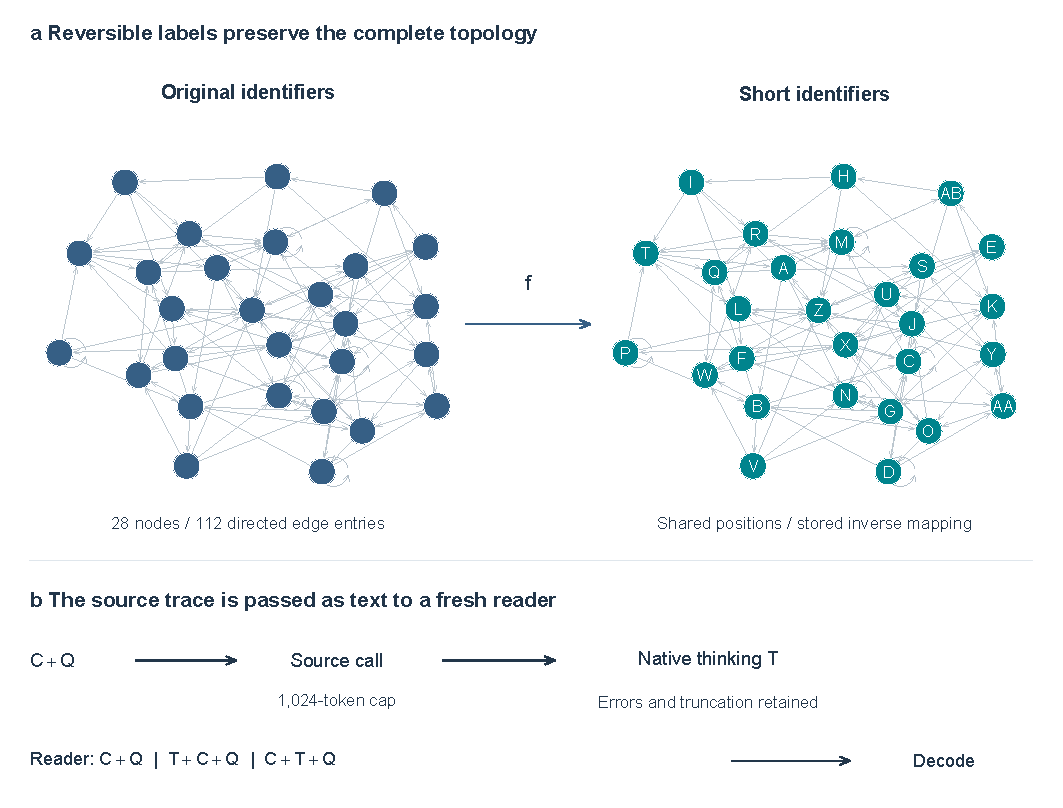
\includegraphics[width=.98\linewidth]{figures/polished_three_20261015/network/publication.pdf}
\caption{Structure-preserving input recoding. (a) Confirmation graph 87 has 28 nodes and 112 directed edge entries. Both views share all vertex positions and edge directions, including five self-loop entries and two repeated edge entries that overlap in the display. Original identifiers are omitted from the left network for legibility; compact labels appear on the right. Positions are display geometry, not learned states. (b) The compact source generates a native thinking block for a fresh reader. Direct, prefix and append orders retain the complete compact context $C$ and final operation $Q$. Prefix and append use byte-identical thinking, including errors and truncation. Inverse mapping restores original labels before scoring. Display geometry does not represent token length.}
\label{fig:method-overview}
\end{figure}

\subsection{Complete compact inputs and single-trace confirmation}
\label{sec:single-trace-method}
\paragraph{Representation and preparation.} This extension changes the original five-trace intervention. A deterministic dictionary replaces each ten-character graph node identifier with a distinct short label that is one token under the archived tokenizer. The same mapping is applied throughout the complete source, examples and question, and its inverse restores predicted nodes. All edges, directions, duplicate edges and operation wording remain available. Exact inverse substitution must reproduce the original prompt; gold answers never determine which content is retained. The label dictionary uses the archived tokenizer, sorted node identifiers and a seeded shuffled vocabulary of one-token uppercase labels, excluding uppercase words already in the prompt; its seed is $202610063+\mathrm{row\_index}$. The inverse dictionary is archived for each graph. A single source pass on the compact input has a 1,024-token output cap. Its entire native thinking field, including mistakes and truncation, is retained in the original warning wrapper; the separate visible answer is excluded. Prefix supplies this block before the compact source, and append supplies the byte-identical block after the source and before the final operation.


\begin{figure}[htbp]
\centering
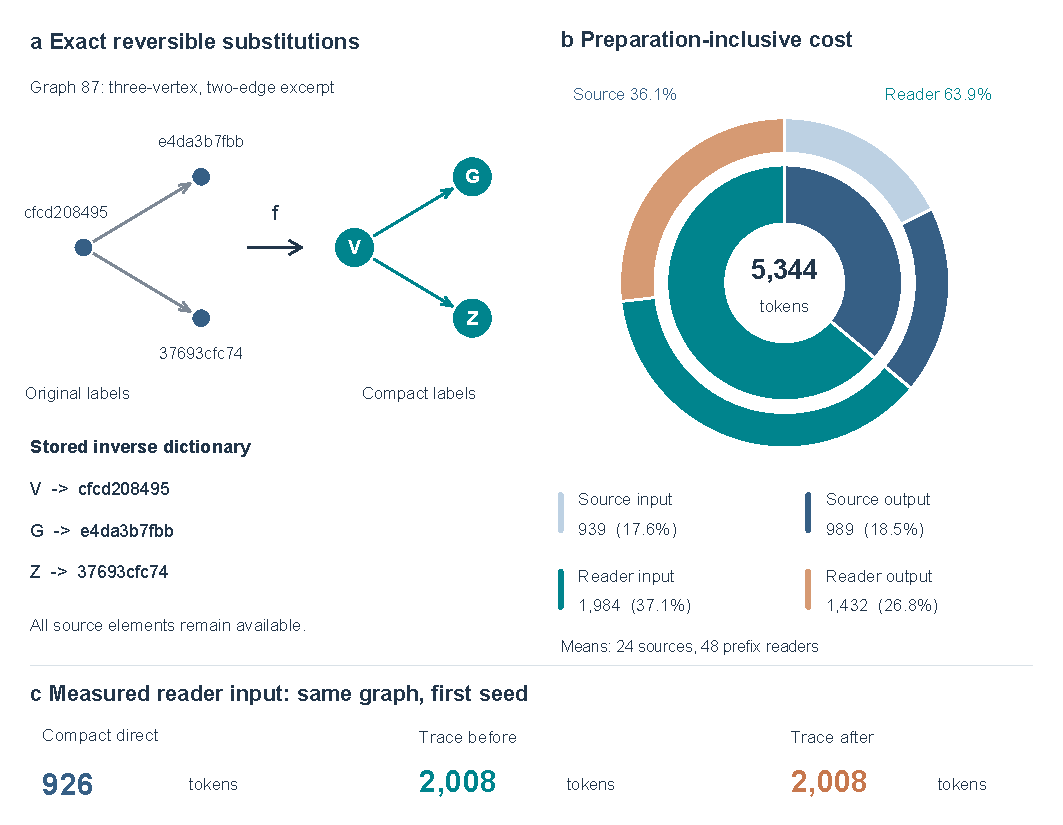
\includegraphics[width=.98\linewidth]{figures/visual_pilot_20261015/method/design.pdf}
\caption{Exact reversible representation and preparation-inclusive token accounting. (a) A three-vertex, two-edge excerpt of confirmation graph 87 before and after recoding; the complete graph has 28 nodes and 112 edge entries. The inverse dictionary restores original identifiers; positions are display geometry. (b) Inner-ring angles split complete mean cost into source and reader usage; outer-ring angles split input and output. Angles alone encode fractions. The total is 5,344.46 tokens per prefix answer, averaged over 24 sources and 48 readers; labels are rounded. Every answer pays full preparation. (c) Native reader input for graph 87's first seed, not population means. Dictionary storage and CPU preprocessing are separate; output caps do not imply matched realized compute.}
\label{fig:method-modules}
\end{figure}

\paragraph{Discovery and confirmation selection.} The discovery study selected twelve previously unused graph heads whose complete original inputs exceeded an 8,192-token contract but whose compact inputs fit, and twelve short graphs in the catalogue interval $[3500,6500)$ characters. Each block contained six parent and six BFS questions. Its 168 calls comprised one source and two readings of each of three arms per graph. The capacity block compared executed original readers at 32,768 context/8,192 output with compact readers at 8,192 context/4,096 output; compact prefix readers reserved 1,024 of that generated-token allowance for preparation. Its predefined practical criterion required a nonempty gold graph to be answered exactly in both compact-direct repeats. Nonexecuted original-8K inputs were feasibility references and were never assigned zero accuracy.

After observing the discovery signal, we froze a separate confirmation using twenty-four new graph heads from the same short catalogue interval, sampled without replacement with twelve questions per task. All archived graph heads, including discovery heads, were excluded. The selection seed was 2026101010, source seed 2026101011 and reader seeds 2026101012--2026101013. Graph order and five-arm order within each repeat were randomized. Each graph supplied one source and ten readers, giving 264 calls. All confirmation calls used Qwen3-1.7B, the archived digest, native thinking, Ollama 0.40.0 and a 32,768-token context. Original and compact direct readers allowed 8,192 generated tokens; the contemporaneous original-long arm allowed 16,384. Prefix and append allowed 7,168 reader tokens after the 1,024-cap preparation pass. These are maximum generated-token allowances, not matched realized compute. Sampling used temperature 0.6, top-$p$ 0.95, top-$k$ 20, minimum-$p$ 0 and repeat penalty 1. Requests were saved before transmission and exact response bytes before parsing. Calls were not retried. Between-call cooling triggered at $82\,^{\circ}\mathrm{C}$ and resumed below $76\,^{\circ}\mathrm{C}$, with three-second call gaps and thirty-second graph-block rests. A corrected discovery cooling implementation and a GPU/reboot interruption are archived; frozen stimuli, model, seeds and budgets were unchanged, and eighteen completed requests were not resent.

\paragraph{Prespecified inference and accounting.} The confirmation primary contrast is prefix minus compact-direct graph-mean F1. Two readings are averaged within each graph; the two task types receive equal weight. The frozen support rule requires a positive mean difference, a positive lower bound of a descriptive stratified graph-bootstrap 95\% interval (20,000 draws; seed 2026101014), and a paired sign-flip Monte Carlo $p\leq0.05$ (100,000 draws; seed 2026101015). The frozen protocol did not specify a test tail; the independent auditor uses the conservative two-sided test, implemented before complete collection and effect analysis. The sign-flip interpretation assumes exchangeability of paired differences under the null. Placement and original-baseline contrasts are secondary and unadjusted for multiple comparisons. The discovery and confirmation results are reported separately, and no outcome-dependent sample extension is used. Each reused answer is charged the entire one-source preparation plus one reader, without dividing preparation across the two reader repeats. Dictionary bytes and CPU recoding time are reported separately. Wall time covers the recorded model requests, not all workflow idle time or preprocessing. A normal-stop terminal visible answer line is required; malformed or length-terminated answers score zero, and unknown inverse labels count as false-positive nodes. Independently recomputed graph gold sets, exact payloads, model/context metadata, token counts and visible responses are audited without importing the runner or its scorer.


\subsection{Reproduction scope and experimental conditions}
Let $x$ denote the graph context, $q$ its operation, and $T$ a serialized block of prior reasoning. Trace prefix and trace append use $[T,x,q]$ and $[x,T,q]$, respectively. Both receive the same realized $T$ and retain the complete original graph. Direct reading uses $[x,q]$; question-first reading uses $[q,x,q]$. Following the original long-context adaptation of Re2 \citep{tang2026trace,xu2024rereading}, we used $[x,q,x,q]$ within one request. A separate fresh request containing $[x,q]$ is not Re2.

The original study used five source traces and five reader repeats, with each reused trace capped at its first 50,000 characters. All completed short-graph placement studies retained this trace count, repeat count and placement comparison. Their local source and reader output limits were 4,096 and 8,192 tokens, respectively. These explicit local limits differ from the original study, which requested no custom client-side output maximum; effective provider defaults were not established. Appendix~\ref{app:reproduction-map} lists the retained and adapted components.

\paragraph{Tasks and selection.} We used the archived 750-row \protect\path{graphwalks_128k_and_shorter.parquet} file from OpenAI GraphWalks \citep{openai2025graphwalks}, comprising 400 parent and 350 BFS questions. This is one file of the released dataset, not its full repository. Its SHA-256 matched the publisher's current file metadata when checked on 6 October 2026. We used directed breadth-first search (BFS) and parent-retrieval tasks. Gold answers were recomputed from graph edges before scoring. Study-specific selection used catalogue length, task type and exclusion of previously selected graph identities. Earlier selection was deterministic. A separate prospective replication randomly selected six new graphs per task from a restricted short-input population; it was not a random sample of all graph questions. Seeds supplied repeated measurements within graphs and did not increase the number of independent graph units.

\paragraph{Models and interfaces.} The reported studies used the nominal Qwen3-1.7B and Qwen3-4B variants \citep{yang2025qwen3} and Qwen3.5-4B \citep{qwen2026qwen35card}, with native thinking exposed separately from visible answers. The main configurations are listed in Table~\ref{tab:local-configurations}. Model digests, runtime versions, sampling settings and complete prompts are preserved in the frozen archives. Native Qwen3.5 studies used Ollama 0.35.1 and a fixed general-thinking profile. Its temperature was 1.0, top-$p$ 0.95, top-$k$ 20 and presence penalty 1.5. The earlier Qwen3 short-trace study used temperature 0.6, top-$p$ 0.95 and top-$k$ 20. These settings were not pooled as a model-size experiment.

\begin{table}[htbp]
\centering\small
\begin{tabular}{>{\raggedright\arraybackslash}p{.33\linewidth}lll}
\toprule
Study & Model & Context & Source / reader cap\\
\midrule
Initial and prospective short studies & Qwen3-1.7B & 32,768 & 4,096 / 8,192\\
Same-question paired follow-up & Qwen3-4B & 32,768 & 4,096 / 8,192\\
Output-budget diagnostic & Qwen3-4B & 32,768 & --- / 28,672\\
Native source qualification & Qwen3.5-4B & 65,536 & 32,768 / ---\\
Native long five-trace trial & Qwen3.5-4B & 131,072 & 32,768 / 32,768\\
Retained-case context diagnostic & Qwen3.5-4B & 196,608 & retained / 32,768\\
Early-state adaptation & Qwen3.5-4B & 65,536 & 1,024 / budget-derived\\
\bottomrule
\end{tabular}
\caption{Token limits for the main local studies. The early-state reader cap was computed separately for each planned request from its fixed total allowance. Context is a configured serving limit, not a measured guarantee of effective reasoning capacity.}
\label{tab:local-configurations}
\end{table}

\paragraph{Prospective short-graph replication.} Before collecting new responses, we froze a twelve-graph protocol and its complete allocation schedule. All graph heads selected in existing official-study freezes were excluded. Within the catalogue interval $[2000,3500)$ characters, the resulting pools contained 34 parent questions and nine BFS questions with distinct graph heads. Six were sampled without replacement per task, using seed 202610060. Graph order and reader-arm order within each repetition were randomized using the same seeded generator. Five source seeds (202610061--202610065) and five matched reader seeds (202610071--202610075) supplied 240 planned calls. Model digest, original serializer, context and source/reader caps matched the initial short study. Decoding used temperature 0.6, top-$p$ 0.95, top-$k$ 20, minimum-$p$ 0 and repeat penalty 1. The native server version was 0.35.1. Complete requests were saved before transmission and exact response bytes before parsing. No call was retried. Sequential calls were separated by five seconds, and graph blocks by sixty seconds. This was a locally frozen prospective protocol, not an external preregistration.

\paragraph{Same-question second-model follow-up.} After observing the 1.7B results, we froze a separate Qwen3-4B study before collecting its 240 new responses. It retained the same twelve questions, graph and arm order, source and reader seeds, complete prompts, sampling parameters and context/output limits. The 4B package generated its own five-trace bundles. This compared local pipelines on matched questions; it did not isolate reader size or supply twelve additional independent graph units. The within-model prefix--append contrast remained primary, with the same descriptive stratified graph bootstrap.

% BEGIN COMPLETE_DIAGNOSTIC_METHODS
\paragraph{Output-budget diagnostic.} Interim 4B output truncation motivated a separately frozen follow-up on the same twelve known questions and five matched reader seeds. Sixty new direct requests used an output cap of 28,672 tokens, equal to $5\times4096+8192$, with all other recorded inputs, model and sampling settings retained. Original 8,192-cap direct responses remained the historical comparator. This matched maximum generated-token allowances, not total logical tokens, memory, time or compute. Conditions ran sequentially; the diagnostic hypothesis was chosen after interim observations. All cases were retained. The descriptive long-minus-original-direct interval used 20,000 stratified graph-bootstrap draws, seed 202610067.

\paragraph{Configured-context diagnostic.} A separate frozen follow-up retained the original five-trace bundle for the previously declined row-506 case. With the original Qwen3.5-4B digest and sampling profile, it changed the configured context from 131,072 to 196,608 tokens. One full-prefix input probe with a one-token output cap checked accounting and residency without scoring an answer. Five paired seeds supplied prefix, append, fresh, question-first and Re2 readers, each with a 32,768-token output cap: 26 new calls in total. Five-second call gaps and sixty-second repeat-block rests were retained. Full original source preparation was charged to trace conditions; new-run usage was separately reported. This deliberately selected failure case diagnosed execution and case-specific outcomes, not a new population sample or completion of the old sixteen-graph trial.

% END COMPLETE_DIAGNOSTIC_METHODS

\paragraph{Trace construction and controls.} Source reasoning was read from the native thinking field; the separate visible answer was excluded. Incorrect and length-terminated source traces were retained according to each frozen protocol. Prefix and append used byte-identical trace blocks. The shorter-state adaptation retained the complete thinking generated under a 1,024-token cap. It did not select excerpts using gold answers. Representation recoding and thinking-mode controls were separate experiments, reported in the appendices.

\subsection{Scoring, qualification and missing outcomes}
For predicted and gold node sets $P$ and $G$, we used
\[
 F_1(P,G)=\begin{cases}
 1,&P=G=\varnothing,\\
 \displaystyle\frac{2|P\cap G|}{|P|+|G|},&\text{otherwise},
 \end{cases}
 \qquad \mathrm{EM}(P,G)=\mathbf{1}\{P=G\}.
\]
Set semantics remove duplicate predictions but retain incorrect nodes. Scoring used visible answers only and never extracted an answer from thinking. Known malformed or length-terminated outputs received zero under their respective protocols. Valid empty answers were scored normally, with an always-empty baseline reported where relevant.

\paragraph{Answer interfaces.} The native source and configured-context studies accepted a valid terminal visible \texttt{Final Answer: [...]} line after a normal stop. The early-state study required that line to constitute the entire visible response. Its later relaxed parser was explicitly post hoc and did not replace the primary scores. Recoding protocols also differed in their treatment of unmapped nodes. Identity recoding invalidated such predictions, whereas indexed-source scoring counted them as false positives. Scores were not pooled across these rules.

\paragraph{Call qualification.} Input counts, response metadata and resident model digest/context were checked against the recorded request. Qualification established compliance with the study's interface, not answer correctness. A qualified response could still be malformed or reach its output limit. A returned response that failed interface qualification remained undetermined under the applicable primary protocol.

\paragraph{Interrupted execution.} Unknown responses were bounded over the original planned denominator, rather than scored as zero or replayed. For $N$ planned outcomes with $m$ unknown values, the F1 bounds were $[\sum F_1/N,(\sum F_1+m)/N]$. Known unsent budget declines were deployment failures, not model answers. Client errors retained their protocol-defined failure scores and unknown usage. Unknown token usage made the reported cost a lower bound.

\subsection{Statistical analysis and resource accounting}
Reader repetitions were averaged within graphs before comparisons across graphs. Intervals condition on the archived trace bundles; independent redraws of complete five-trace bundles were not sampled. The short-trace study used 20,000 graph bootstrap resamples, seed 202610040, for descriptive 95\% percentile intervals. Its four graphs did not support a broad population claim. The twelve-graph replication specified prefix-minus-append F1 as its primary contrast and prefix-minus-direct as secondary. Each task stratum contributed equally. Its descriptive percentile intervals used 20,000 bootstrap draws of six graph units within each task stratum, seed 202610066. All twelve selected graphs and all repeated outcomes were included, without score-dependent stopping. Subsequent studies retained their own frozen analysis families and screening criteria (Appendix~\ref{app:gate-map}). These criteria governed advancement to further research; they were not universal definitions of successful replication or formal noninferiority tests.

Deployment-token accounting included the complete source inputs and outputs plus one reader's input and output. Repeated reader calls estimated that reader cost; they did not divide the preparation bill. Research-run totals were reported separately and included calibration where performed. Token accounting did not establish latency, energy or cache-related computation savings. The prospective replication separately recorded observed request wall times, without an exclusive-hardware or comparative-latency claim. A dedicated API endpoint also did not establish exclusive hardware use.

\section{Results}
\subsection{Compact inputs and a short trace improved accuracy on independent new graphs}
\label{sec:confirmed-benefit}
All 264 confirmation calls completed and were independently audited, with no unknown responses. Of the twenty-four source passes, twenty-two ended at the 1,024-token output limit; the two normally stopped visible source answers were valid but incorrect. None of the source passes produced a correct qualified visible answer. Their unfiltered thinking was nevertheless retained, so the observed reader benefit does not require a correct source answer under this short cap. Prefix F1 increased from compact-direct 0.6542 to 0.7703: a difference of 0.1161 (descriptive 95\% interval $[0.0437,0.1914]$; two-sided sign-flip $p=0.00624$). This met the frozen primary support rule on the twenty-four independent graph units. Exact match increased from 0.2292 to 0.3750 as a secondary descriptive outcome. The benefit belongs to the complete trace package, including its warning wrapper and preparation, rather than to placement alone.

\begin{table}[htbp]
\centering\small
\begin{tabular}{lrrrrr}
\toprule
Confirmation arm & F1 & EM & Full tokens/answer & Valid/48 & Length\\
\midrule
Original direct & 0.3176 & 0.0417 & 6,640.67 & 43 & 5\\
Original direct, 16K output & 0.3668 & 0.0833 & 7,149.88 & 45 & 3\\
Compact direct & 0.6542 & 0.2292 & 3,823.25 & 42 & 6\\
Compact trace prefix & 0.7703 & 0.3750 & 5,344.46 & 47 & 1\\
Compact trace append & 0.7130 & 0.3333 & 5,345.67 & 46 & 2\\
\bottomrule
\end{tabular}
\caption{Independent confirmation on twenty-four new graphs, two reader seeds per graph. F1 and EM average within graphs before aggregation. Full model tokens include complete preparation for each reused answer. Every length-terminated reader is included with zero score. ``Valid'' denotes answer-format validity after a normal stop, not correctness. All arms used the same 32K configured context.}
\label{tab:confirmation-benefit}
\end{table}

\subsection{The accuracy benefit incurred a cost relative to compact direct reading}
Prefix used 1.398 times the complete model tokens of compact direct reading (descriptive interval $[1.170,1.667]$). Its wall-time ratio was 0.842, but its interval $[0.630,1.119]$ included one. Thus the primary benefit was higher accuracy with additional tokens; faster execution than compact direct was not established.

Against original direct, prefix F1 was higher by 0.4527 (interval $[0.3320,0.5656]$) and its full-token ratio was 0.805 (interval $[0.724,0.896]$). Against original-long, the F1 difference was 0.4034 (interval $[0.2931,0.5087]$) and the token ratio was 0.747 (interval $[0.635,0.877]$). These prespecified secondary comparisons include both recoding and trace reuse. Compact direct itself improved F1 over original direct by 0.3366 (interval $[0.1932,0.4759]$), with a token ratio of 0.576 (interval $[0.466,0.711]$). The combined improvement cannot be assigned entirely to traces.

The matched prefix-minus-append F1 difference was 0.0573 (interval $[-0.0321,0.1705]$; $p=0.36592$), leaving placement superiority uncertain. Append minus compact-direct was also uncertain: 0.0588 (interval $[-0.0600,0.1695]$). Secondary intervals are descriptive and unadjusted for multiplicity. Figure~\ref{fig:benefit-confirmation} displays quality, preparation-inclusive model tokens and paired graph-level uncertainty.

\begin{figure}[htbp]
\centering
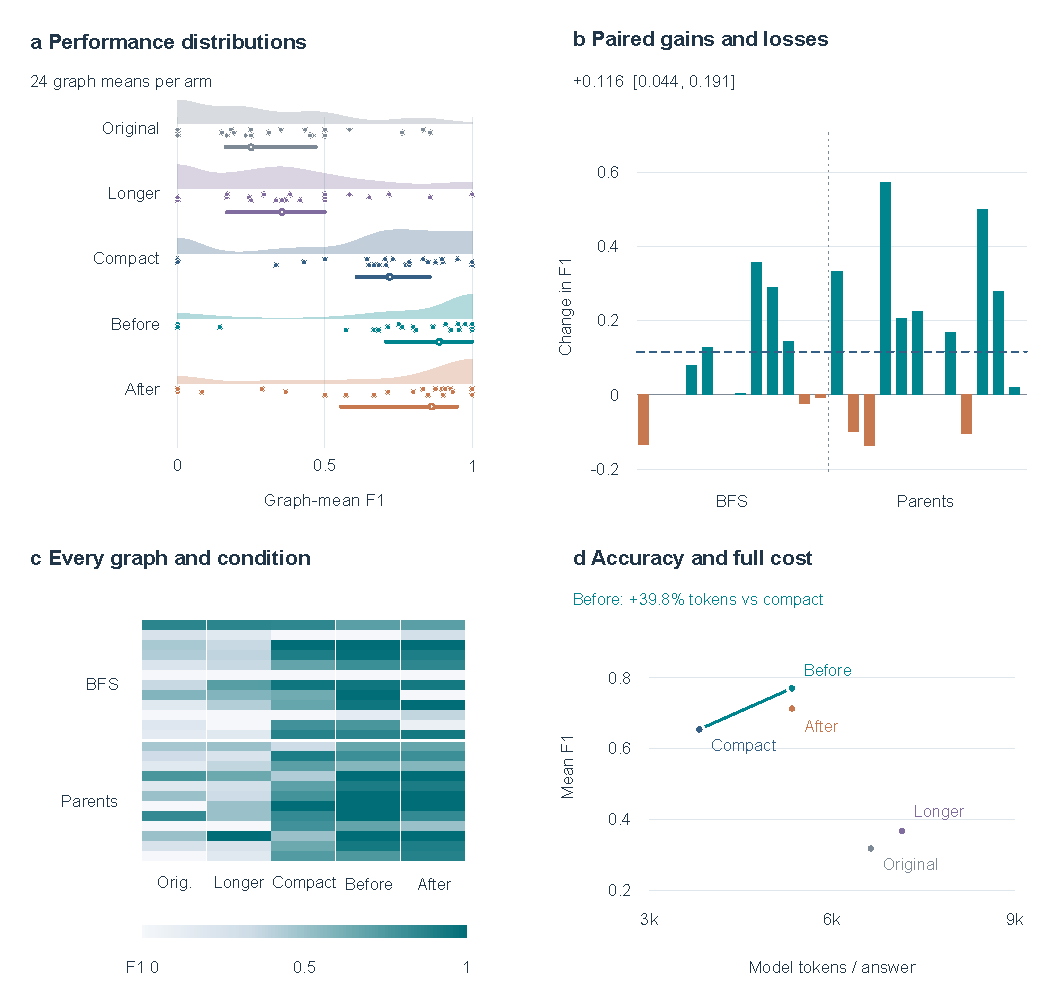
\includegraphics[width=.98\linewidth]{figures/polished_three_20261015/confirmation/publication.pdf}
\caption{Independent single-trace confirmation across twenty-four graph units, with two reader seeds averaged within each graph. (a) All graph-mean F1 values; shaded densities are descriptive boundary-reflected estimates with bandwidth 0.08 and heights normalized within each arm. Horizontal segments show interquartile ranges and white markers show medians. (b) Prefix-minus-compact differences for every graph in fixed order within task; teal and orange denote gains and losses. The dashed horizontal line is the mean difference; the stated 95\% interval is the prespecified stratified graph-bootstrap interval. Zero differences have zero-height bars. Before and after denote prefix and append; longer denotes the original-input larger-output control. (c) All 120 graph--method outcomes on a common F1 scale, using the same task-grouped order as (b). (d) Mean F1 versus complete model tokens per answer, charging the entire source preparation to each trace answer. The connecting segment identifies the primary comparison, not a continuous performance curve. Prefix improves mean F1 at 39.8\% more full tokens than compact direct. Other comparisons remain secondary and unadjusted for multiplicity; placement superiority remains uncertain.}
\label{fig:benefit-confirmation}
\end{figure}


\label{sec:migration-results}
\subsection{Discovery and capacity boundaries}
The discovery's short-graph prefix-minus-compact F1 difference was 0.1534, with a descriptive interval $[0.0394,0.2769]$. This was an exploratory contrast, motivating the independent confirmation rather than serving as its evidence. The capacity block did not meet its practical criterion: no nonempty gold graph was answered exactly in both compact-direct repeats, although all twelve compact inputs fit the 8K contract (Figure~\ref{fig:benefit-discovery}). Input fit alone therefore did not establish successful task capacity.

\begin{figure}[htbp]
\centering
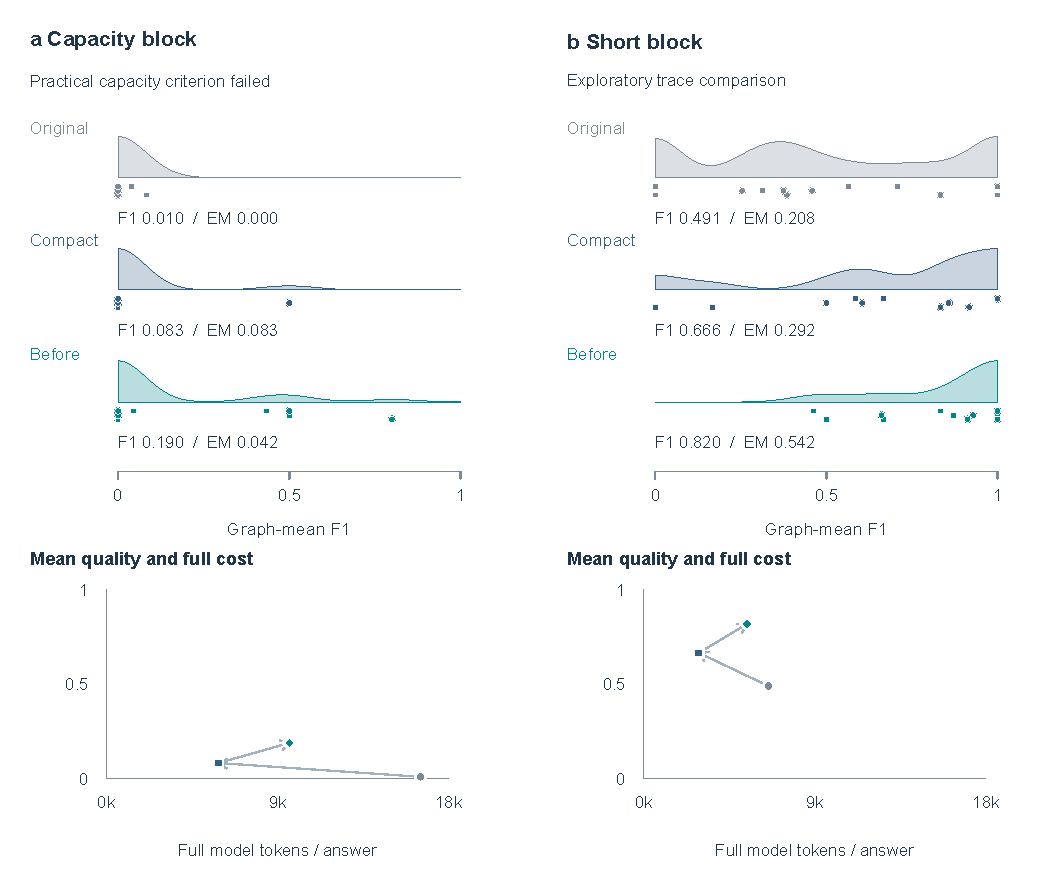
\includegraphics[width=.98\linewidth]{figures/refined_r_20261015/user_benefit/publication.pdf}
\caption{Discovery study, separate from confirmation. Each block retains twelve graph means, with two reader repeats averaged within graphs; circles denote parents and squares BFS. Descriptive boundary-reflected F1 densities use bandwidth 0.08 and equal peak height; all observations remain visible. Printed values give F1/EM means. Below, arrows connect original, compact and prefix arm means in that order; circles, squares and diamonds identify these arms. Score and complete-token scales are shared across blocks. Costs charge full preparation. Capacity packages have different serving allowances; complete original inputs would not fit the nonexecuted 8K reference. Input fit did not meet the predefined nonempty exact-in-both-repeats practical criterion. Short-block results are exploratory.}
\label{fig:benefit-discovery}
\end{figure}


\subsection{Prospective replication left the placement advantage uncertain}
\label{sec:prospective-replication}
The twelve-graph follow-up completed all 240 planned calls: sixty sources and sixty reader responses per condition. Every call passed the recorded interface checks; none was declined for context or had unknown usage. Twelve sources reached their 4,096-token limit. Prefix and append each produced sixty normal-valid visible answers, compared with 59 for direct reading; the remaining direct response reached its output limit. Incorrect and truncated source reasoning remained in the shared trace block.

Mean F1 was 0.7715 for prefix, 0.7351 for append and 0.6915 for direct reading (Figure~\ref{fig:prospective-replication}). The primary prefix-minus-append difference was 3.64 percentage points, with a descriptive interval of $[-0.65,8.33]$ points. The secondary prefix-minus-direct difference was 8.00 points, interval $[-3.00,17.98]$ points. Both intervals included zero. EM was 0.3333, 0.3833 and 0.3333 respectively: the higher prefix F1 did not extend to exact match. Two graphs had empty gold answers; an always-empty response therefore scored 0.1667 in both metrics over this sample.

The prefix-minus-direct F1 point difference was $+20.79$ points for parents but $-4.80$ points for BFS. These six-graph strata did not establish a task-specific causal mechanism. They showed why an aggregate positive point estimate should not be described as a uniform improvement. The follow-up remained separate from the initial four graphs; their scores and intervals were not pooled.

Charging all five source calls plus one seed-averaged reading gave mean deployment costs of 34,901.15 tokens for prefix, 34,622.07 for append and 4,093.48 for direct reading. Prefix cost $8.53$ times direct reading under this single-question contract. The complete research run consumed 2,308,239 model tokens. Observed request wall times summed to 4,115.32 seconds, excluding the planned idle gaps; this was neither total elapsed deployment time nor a hardware-exclusive latency comparison.

\begin{figure}[htbp]
\centering
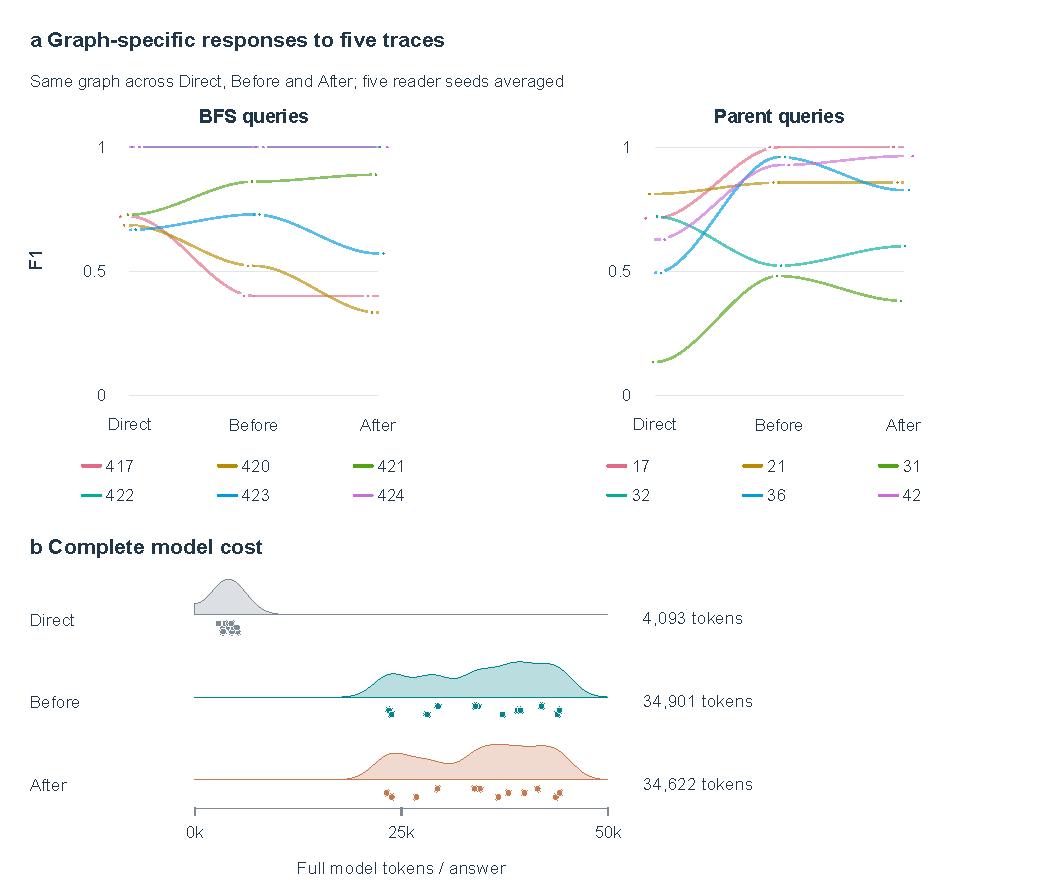
\includegraphics[width=\linewidth]{figures/refined_r_20261015/official_graph_confirmatory_20261006/publication.pdf}
\caption{Prospective twelve-graph replication from independently rescored responses. (a) Curves track the same graph across direct, front-trace and back-trace conditions, separately for BFS and parent queries. Colours and identifiers distinguish graphs; smooth connections interpolate only between discrete conditions. F1 averages five reader seeds. Horizontal marker offsets separate coincident scores without changing F1. (b) All twelve complete-token graph means per arm with descriptive zero-reflected densities, bandwidth 2,000 and equal peak height; printed values are means. Trace answers pay all five sources and one reader, direct answers only the reader. All 240 calls completed; format and termination failures retain prescribed zero scores. Both empty-gold graph units remain in all analyses. Paired contrasts and existing descriptive intervals are reported in the text and tables.}
\label{fig:prospective-replication}
\end{figure}

% BEGIN COMPLETE_PAIRED_NUMERIC_TABLE
\begin{table}[htbp]
\centering\small
\begin{tabular}{lrrrr}
\toprule
Configuration & F1 & EM & Normal-valid & Tokens/answer\\
\midrule
1.7B prefix & 0.7715 & 0.3333 & 60/60 & 34,901\\
1.7B append & 0.7351 & 0.3833 & 60/60 & 34,622\\
1.7B direct & 0.6915 & 0.3333 & 59/60 & 4,093\\
4B prefix & 1.0000 & 1.0000 & 60/60 & 51,751\\
4B append & 1.0000 & 1.0000 & 60/60 & 51,612\\
4B direct & 0.6967 & 0.6833 & 42/60 & 8,231\\
\bottomrule
\end{tabular}
\caption{Completed Qwen3 comparisons on the same twelve graphs, five reader repeats each. Trace costs charge all five sources and one reader. Normal-valid refers to termination and visible-answer format, not correctness. The same questions are not twenty-four independent graph units.}
\label{tab:paired-final}
\end{table}


% END COMPLETE_PAIRED_NUMERIC_TABLE

\subsection{The second model reached a ceiling in both trace placements}
\label{sec:paired-models}
The same-question Qwen3-4B follow-up completed all 240 planned calls and passed independent request, token-count, runtime and scoring checks. Prefix and append each gave sixty normal-valid and exact answers: mean F1 and EM were both 1.0000 (Figure~\ref{fig:paired-models}). All sixty source calls reached the 4,096-token limit and therefore had zero visible-answer scores. Their thinking was nevertheless retained according to the frozen rule. Successful second-pass answering with supplied traces did not require a completed correct visible source answer under this budget.

Direct reading achieved F1 0.6967 and EM 0.6833. Eighteen of sixty direct responses reached the 8,192-token limit; forty-two stopped normally with valid terminal answers. Prefix minus direct F1 was 30.33 percentage points, with a descriptive interval of $[13.67,46.67]$ points. The task-stratum differences were $+0.67$ points for parents and $+60.00$ points for BFS. This pipeline contrast included additional reasoning, warning instructions and preparation calls, and could be affected by direct-output truncation. It did not isolate a placement effect or a same-total-budget advantage.

The primary prefix--append contrast was exactly zero on every graph. Its bootstrap interval collapsed to zero because both conditions were at the observed score ceiling, not because population equivalence had been established. The supplied-trace conditions answered these questions reliably, while leaving no observed preference for front placement. This observation did not by itself establish how the reader used the traces. Cross-model differences also included separately generated trace content, rather than reader size alone.

Preparation-inclusive mean tokens per answer were 51,751.22 for prefix, 51,611.63 for append and 8,231.05 for direct reading. Prefix required $6.29$ times the direct tokens. The complete research run used 3,740,754 model tokens; observed request-wall times summed to 15,435.86 seconds, excluding planned rests. These were logical usage and observed timings, not energy or hardware-exclusive latency measurements.

\begin{figure}[htbp]
\centering
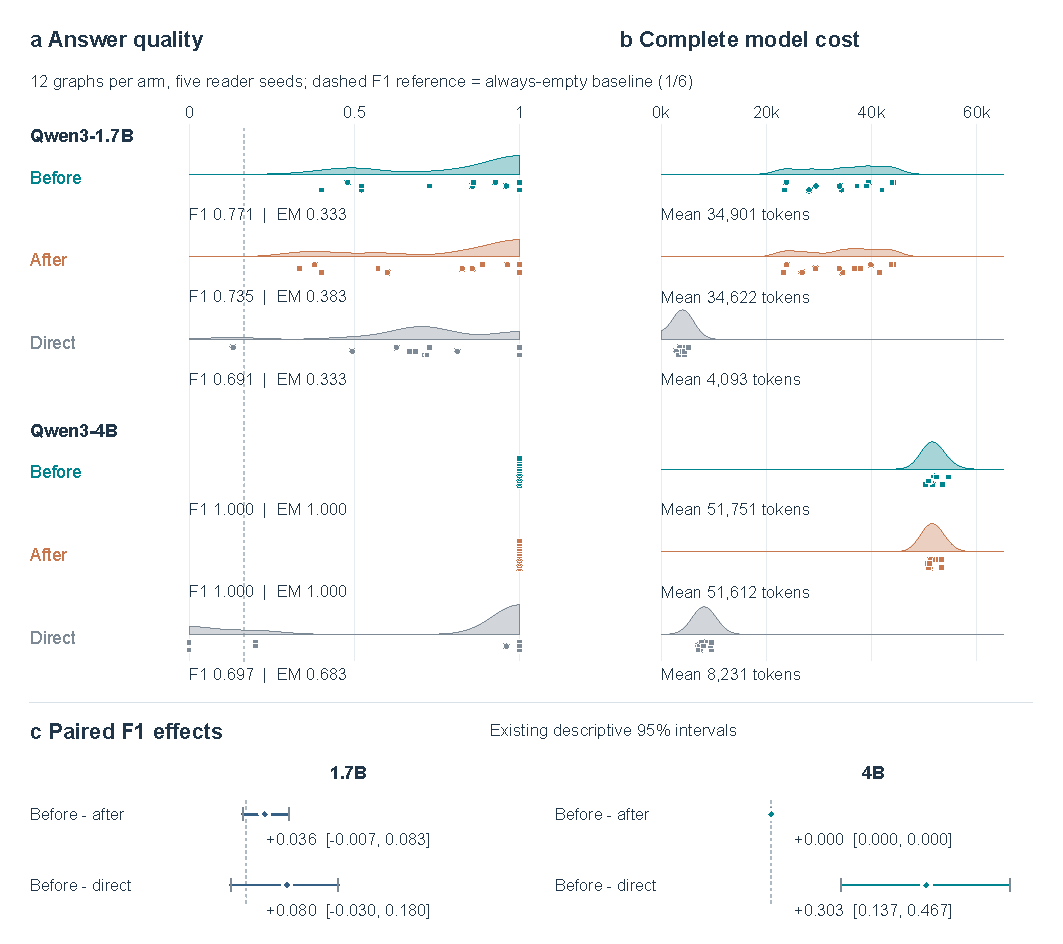
\includegraphics[width=\linewidth]{figures/visual_pilot_20261015/models/design.pdf}
\caption{Qwen3 packages on the same twelve questions, five reader seeds per graph, from two separately audited 240-call studies. (a,b) All graph means: circles denote parents, squares BFS. Perpendicular offsets separate observations. Shaded curves are descriptive densities (F1 reflected at both bounds, bandwidth 0.08; tokens reflected at zero, bandwidth 2,000), with common height scales within metrics. Ceiling conditions retain all twelve observations without smoothing. F1/EM means are printed; the dashed reference is always-empty F1. Costs charge all five sources and one reader. (c) Existing descriptive stratified graph-bootstrap intervals; dashed lines denote zero. The 4B zero-width placement interval reflects the observed ceiling, not population equivalence. Packages generate their own traces; this is not a size-only comparison. Eighteen length-terminated 4B direct readings retain zero scores.}
\label{fig:paired-models}
\end{figure}

% BEGIN COMPLETE_OUTPUT_BUDGET_RESULTS
\subsection{A larger output allowance was tested on the same questions}
\label{sec:output-budget}
All sixty new direct-long calls completed and passed independent request and scoring checks. With a 28,672-token output cap, mean F1 was 1.0000, EM 1.0000, and 60/60 responses were normal-valid. There were 0 length-terminated outputs, compared with eighteen under the original cap. The paired F1 change from the original direct condition was 30.33 percentage points, with a descriptive interval of $[13.33,46.67]$ points. These results quantify this sequential diagnostic on the known questions, rather than a fresh-case or equal-compute comparison.

Mean logical tokens for one direct-long answer were 8,763.78, compared with 8,231.05 in the original direct condition. The new diagnostic incurred 525,827 model tokens and 5,912.53 seconds of observed request time, excluding planned rests. The original trace scores and costs were not overwritten. Prefix preparation cost was 5.91 times direct-long tokens, with the same observed F1 and EM ceiling.

Among the eighteen previously length-terminated responses, 0/18 new thinking strings began with the old thinking text with trailing whitespace removed. The new runs were therefore not byte-identical continuations of the old runs despite matching seeds. This descriptive check further limits attribution of every changed answer to the output cap alone.

\begin{table}[htbp]
\centering\small
\begin{tabular}{lrrrr}
\toprule
Output cap & F1 & EM & Normal-valid & Tokens/answer\\
\midrule
8192 & 0.6967 & 0.6833 & 42/60 & 8,231\\
28672 & 1.0000 & 1.0000 & 60/60 & 8,764\\
\bottomrule
\end{tabular}
\caption{Sequential Qwen3-4B diagnostic on the same known questions and seeds. The larger cap equals the five-source pipeline maximum generated-token allowance, not its total logical-token or compute budget. Original 8192-cap responses remain unchanged.}
\label{tab:budget-final}
\end{table}


\begin{figure}[htbp]
\centering
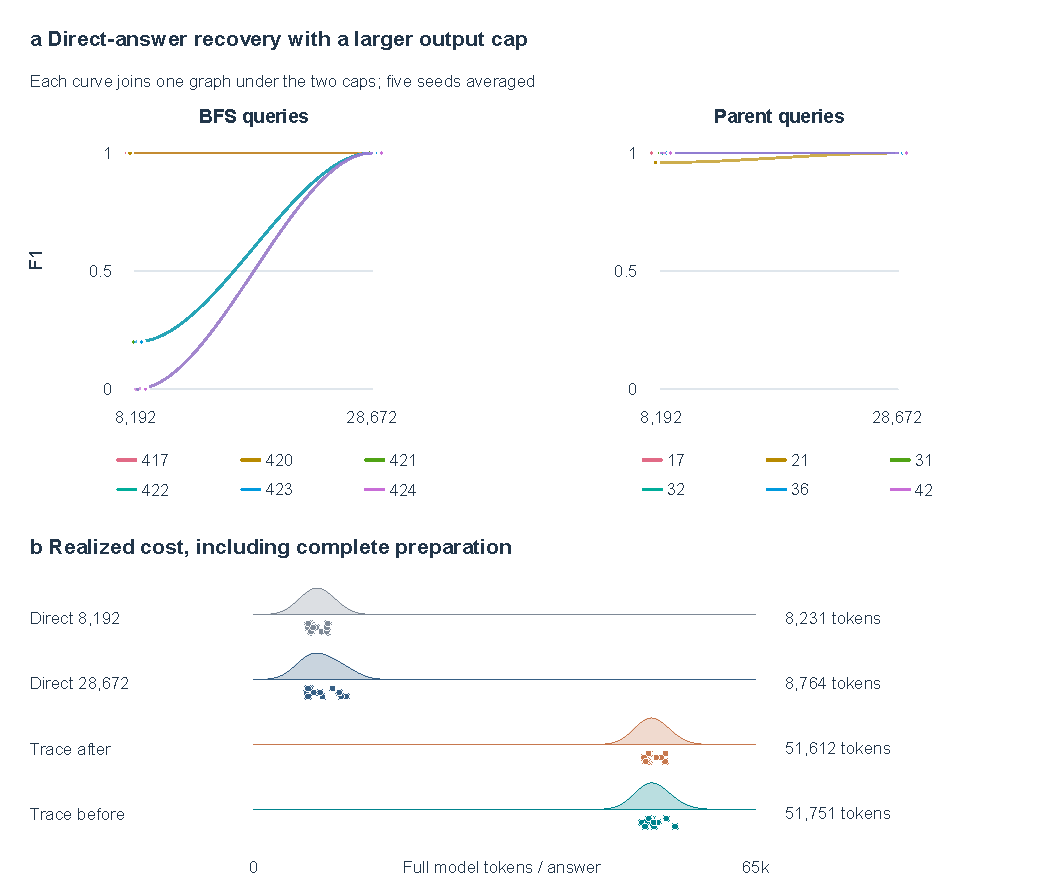
\includegraphics[width=\linewidth]{figures/refined_r_20261015/output_budget_20261006/publication.pdf}
\caption{Sequential output-cap diagnostic on the same twelve Qwen3-4B questions. (a) Each colour tracks one identified graph under direct-output caps of 8,192 and 28,672, with five seeds averaged. Curves interpolate between discrete conditions only; horizontal marker offsets expose overlapping ceiling observations without changing F1. Old length-terminated responses retain zero scores. (b) All twelve complete-token graph means per condition and descriptive zero-reflected densities (bandwidth 2,000, equal peak height); printed totals are means. Trace costs include all five sources. New direct answers and both trace placements reach the observed F1/EM ceiling. This known-question diagnostic matches maximum generated allowances, not total compute, and establishes neither population equivalence nor isolated causality.}
\label{fig:output-budget}
\end{figure}

% END COMPLETE_OUTPUT_BUDGET_RESULTS

\subsection{Native source qualification succeeded on the selected graphs}
A separately frozen Qwen3.5-4B experiment tested source answering with a larger context and output allowance. Earlier bridge archives are retained for selection lineage but excluded from empirical claims because their transmitted-request provenance is weaker (Appendix~\ref{app:reproduction-map}).

With a 65,536-token context and 32,768-token source output cap, all sixteen source calls stopped normally and met qualification. Across eight new graphs, F1 was 0.9286 and EM was 0.875. Figure~\ref{fig:hybrid-source} shows that errors remained on a long-BFS graph. The source screening criterion passed, providing a qualified starting point for the next migration trial. These calls did not test second-pass trace reuse.

\begin{figure}[htbp]
\centering
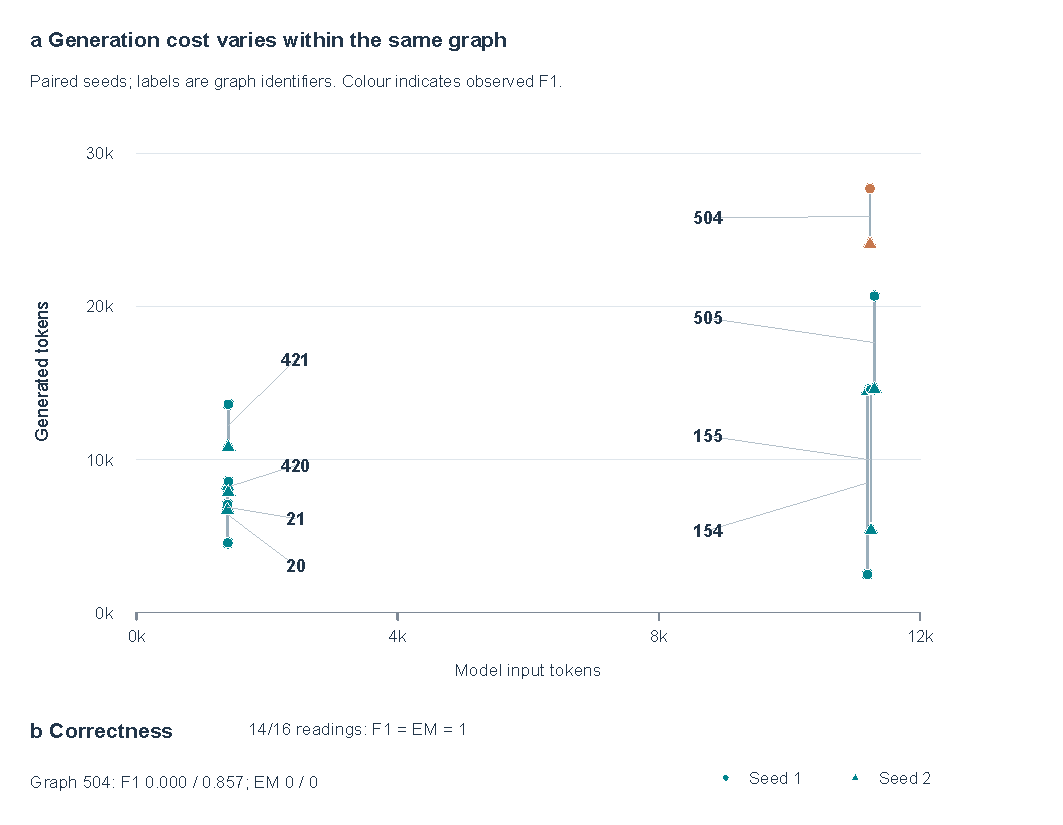
\includegraphics[width=.98\linewidth]{figures/refined_r_20261015/source_qualification_figure/publication.pdf}
\caption{Native source qualification on eight official graphs and two repeats, excluding calibration. (a) Every saved call is located by its input and generated tokens. Circles and triangles distinguish seeds; connectors join repeats of the same identified graph, not a fitted relationship. Teal denotes F1 equal to one and orange lower F1. Thin leader lines connect identifiers to pair midpoints. (b) Fourteen readings have F1 and EM equal to one; graph 504 has F1 0 and 0.857 and EM 0 for both seeds. All points have fixed size; no inferential error bars are shown. No trace reuse was tested.}
\label{fig:hybrid-source}
\end{figure}

\subsection{Five native traces exceeded the configured reader context}
The next trial planned sixteen long-BFS graphs, five sources per graph and five repeats of five reader conditions. On the first graph, prefix and append each required 144,677 input tokens. This exceeded the configured 131,072-token context before any reader output was generated (Figure~\ref{fig:hybrid-interrupted}). Both trace conditions were declined under the frozen resource rule, without shortening their trace block.

The trial subsequently stopped after a returned response failed its resident-model check. Of 480 planned formal slots, fourteen returned qualified responses, eight were budget declines, one returned response was unqualified, and 457 were unreached. These categories preserved 22 determined deployment outcomes and 458 unknown outcomes. The archive established first-graph infeasibility under the specified configuration, but not a sixteen-graph quality effect.

The frozen inputs also permitted a conditional cost calculation. Let $I$ be one complete source input and $C$ the direct output allowance. Five source inputs alone cost $5I$, whereas one direct prediction costs at most $I+C$. Hence
\[
 I>C/4\quad\Longrightarrow\quad 5I>I+C.
\]
All sixteen planned inputs satisfied $I>8192$ with $C=32768$. Under this single-prediction accounting contract, five complete sources could not be cheaper than direct reading. This bound did not apply to latency, caching, different output caps or preparation reused across different questions.

\begin{figure}[htbp]
\centering
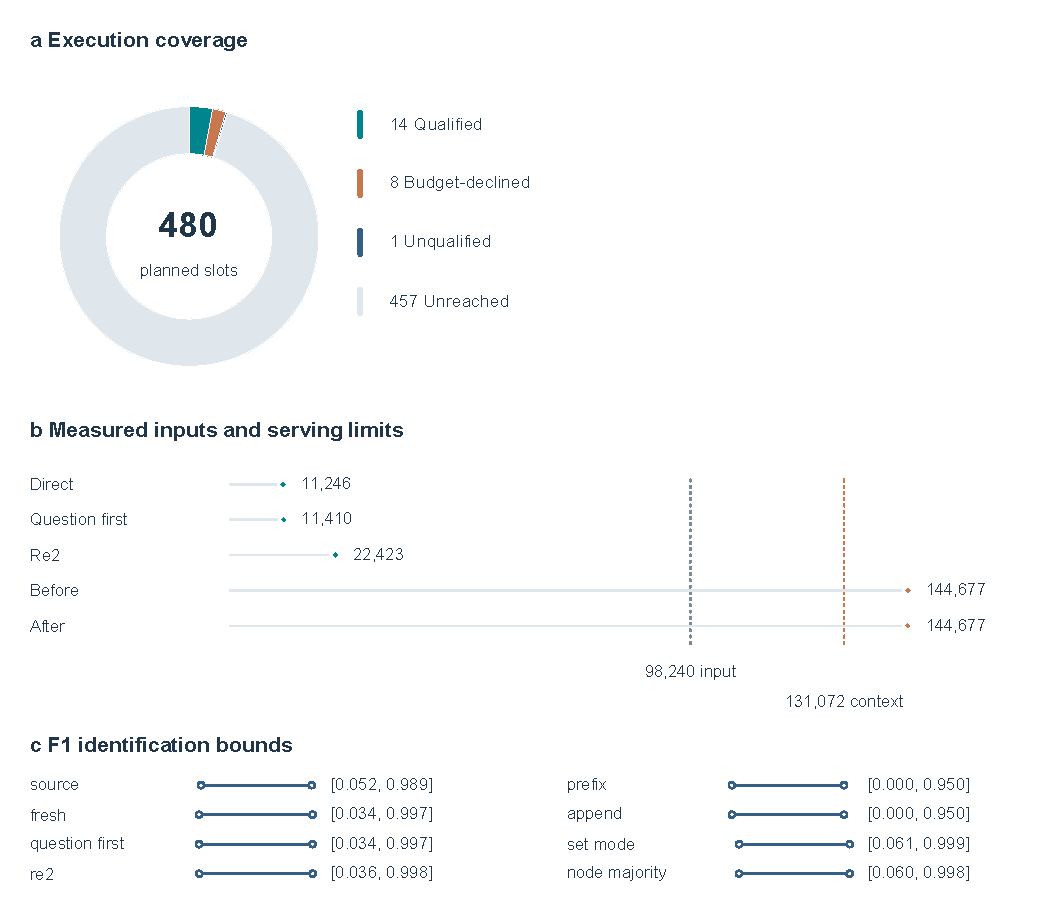
\includegraphics[width=\linewidth]{figures/refined_r_20261015/interrupted_study_figure/publication.pdf}
\caption{Context and execution boundaries of the native five-trace trial. (a) Annular angles partition all 480 formal slots, excluding calibration, into qualified responses, budget declines, unqualified responses and unreached slots; counts are printed. Unreached slots are not failed answers. (b) Measured first-graph inputs against the input limit after output reservation (98,240) and configured context (131,072), shown by dashed thresholds. (c) Open endpoints delimit F1 identification bounds over all sixteen planned graph outcomes; numeric labels give both endpoints. These are not confidence intervals. Missing outcomes prevent a quality conclusion.}
\label{fig:hybrid-interrupted}
\end{figure}

% BEGIN COMPLETE_CONTEXT_DIAGNOSTIC_RESULTS
\subsection{A larger configured context enabled the retained-case diagnostic}
\label{sec:context-diagnostic}
All twenty-six new calls passed independent request, input-count and resident-model checks at a configured 196,608-token context. The probe verified the full 144,677-token prefix input; it was not a scored answer. This established execution at the changed allocation for this case, rather than reasoning capacity throughout the context window.

Across five reader seeds, prefix F1/EM were 0.9750/0.8000, append 0.8984/0.6000, and fresh direct reading 0.9583/0.4000. Normal-valid counts were 5/5, 5/5 and 5/5 respectively. Table~\ref{tab:context-final} retains all five conditions. No population interval was inferred from this deliberately selected case. The old sixteen-graph archive remained interrupted and its unknown outcomes were not replaced.

The original five-source preparation cost was 190,884 tokens. New probe and reader calls consumed 2,343,997 model tokens, with 12,135.52 seconds of observed request time. Preparation was charged once to each trace deployment estimate, never amortized over the five experimental repeats.

\begin{table}[htbp]
\centering\small
\begin{tabular}{lrrrr}
\toprule
Reader & F1 & EM & Normal-valid & Tokens/answer\\
\midrule
prefix & 0.9750 & 0.8000 & 5/5 & 350,021\\
append & 0.8984 & 0.6000 & 5/5 & 344,816\\
fresh & 0.9583 & 0.4000 & 5/5 & 36,498\\
question first & 0.7220 & 0.0000 & 5/5 & 39,719\\
re2 & 0.7692 & 0.6000 & 4/5 & 50,578\\
\bottomrule
\end{tabular}
\caption{One previously selected overflow case, evaluated at a configured 196608-token context with the original trace bundle. Five repeats per condition describe this case only; no population interval is inferred. Prefix and append include the complete original source preparation cost.}
\label{tab:context-final}
\end{table}


% END COMPLETE_CONTEXT_DIAGNOSTIC_RESULTS

\subsection{Answer-format sensitivity limited the early-state comparison}
A separately frozen adaptation used a 1,024-token source cap and seven reader conditions with a shared total-token allowance. Execution remained incomplete, with 129 of 224 planned reader outcomes known. Under a post hoc parser that accepted a valid terminal answer within surrounding prose, prefix, direct and question-first reading each produced thirteen exact answers on eighteen matched outputs. The primary strict scores were retained. This sensitivity showed that an apparent strict-score advantage could depend on format compliance; it did not establish equivalence or a placement benefit. Appendix~\ref{app:early-state-detail} reports the planned-denominator bounds, failures and resource accounting.

\subsection{Additional controls identified separate sources of variation}
The initial four-graph Qwen3-1.7B study also favored prefix in mean F1, but both paired descriptive intervals included zero. Appendix~\ref{app:initial-short-study} retains its full numerical results and preparation cost; it is not pooled with the prospective twelve-graph follow-up.

Representation and decoding studies tested interventions distinct from trace placement. Reversible compact node names improved the F1 point estimate by 15.23 points and reduced tokens by 50.46\%. Its eight-graph interval against original names was $[-21.15,40.98]$ points, leaving the quality effect uncertain. Thinking-off and a fixed task route reduced tokens while lowering quality (Appendix~\ref{app:representation-controls}).

The indexed-source study saved 94 of 96 planned responses. Its primary indexed-off candidate failed the frozen criterion. A secondary compact-on comparison remained positive under worst-case missing-score bounds, but unknown usage prevented a complete cost comparison (Appendix~\ref{app:indexed-source}). Small longer-input and sampling studies also showed sensitivity to decoding and empty-answer baselines. They did not identify a single causal sampling parameter or a universal long-input failure.

\section{Discussion}
The studies distinguish a confirmed small-model accuracy benefit from placement superiority and universal efficiency. In the independent compact-input confirmation, a single front trace improved F1 with an additional token cost relative to compact direct reading. Secondary original-input comparisons showed a favorable quality--token trade-off, including against a contemporaneous larger-output baseline. The original five-trace reproduction did not establish that preparing and reusing reasoning lowered the token cost of one accurate answer. This deployment question must be separated from whether supplying traces improves an answer under a particular reader cap. The initial and prospective Qwen3-1.7B studies favored trace prefix in mean F1, but both descriptive placement intervals included zero. The twelve-graph study also showed lower prefix EM than append and opposing prefix-versus-direct point differences across tasks. On the same questions, Qwen3-4B reached perfect F1 and EM in both trace placements; its direct condition was substantially affected by output truncation. Thus answering with supplied traces and a front-placement advantage were different empirical questions. The native source study showed that selected graph questions could be answered reliably under a different configuration. It did not establish that a reader would benefit from those traces.

% BEGIN COMPLETE_DIAGNOSTIC_DISCUSSION
In the output-budget diagnostic, direct F1 was 1.0000 versus 0.6967 in the earlier run, with the same questions and sampling settings. The prefix preparation-inclusive token bill was 5.91 times that of the new direct condition at the same observed accuracy ceiling. Because its hypothesis was selected after truncation and conditions ran sequentially, it supports a bounded output-budget interpretation, not a pure causal estimate of the reasoning-state mechanism. The retained-case context diagnostic also separated a configured allocation failure from execution at a larger allocation; it did not fill the old trial's missing quality outcomes.

% END COMPLETE_DIAGNOSTIC_DISCUSSION

\paragraph{Relation to Trace as State.} The original method supplies prior reasoning before an unchanged source, allowing it to guide rereading \citep{tang2026trace}. Our placement comparison retained that intervention. Differences in models, task lengths, output limits and interfaces prevented a direct comparison with the original benchmark scores. The local uncertainty therefore did not contradict the reported frontier-model result. The original paper also acknowledged additional latency and token costs; our accounting quantified a particular local configuration rather than identifying a flaw overlooked by its authors.

\paragraph{Separating the constraints.} Source competence, reader feasibility and placement benefit are distinct questions. A successful source pass answers only the first. Conversely, an incorrect or incomplete source answer does not rule out useful intermediate reasoning: source correctness is not a prerequisite for testing reuse. Context overflow prevents the second pass from testing placement at all. Output-format sensitivity limits interpretation of a measured score difference. Treating these conditions separately prevents an execution failure or parsing difference from being mistaken for a failure of the underlying reasoning principle.

\paragraph{Implications for low-cost inference.} In these graph configurations, the larger-output direct diagnostic achieved the same observed 4B accuracy ceiling as the trace conditions with a smaller preparation-inclusive token bill. This is a sequential, known-question diagnostic, not an equal-compute or purely causal comparison. It motivates checking whether a direct baseline has sufficient output allowance before attributing a pipeline advantage to reuse. A lower-cost trace pipeline would also need to reduce or amortize its preparation; the present traces were question-specific, and cross-question amortization was not measured. Token usage does not by itself establish latency, energy or monetary savings.

\paragraph{Implications for further reproduction.} Further long-input reproduction should first ensure that the intended trace block and output reserve fit every selected input. It should then compare identical trace content before and after the source with paired graph measurements. Semantic correctness, strict output compliance and truncation should be specified separately before collection. Fewer traces or compressed traces change the intervention and require their own matched controls. These are prospective requirements, not additional findings of this study.

\paragraph{Contribution of the boundary study.} The primary contribution is a local accuracy--cost assessment grounded in a reproduction of the placement intervention. The evidence identifies qualified source configurations, cases where the intended second pass was declined under its configured resource contract, and a scoring confound requiring explicit control. It narrows the conditions for a meaningful small-model test. The new compact-input confirmation adds a prespecified accuracy benefit for a single-trace package; it remains separate from the original five-trace placement evidence. Earlier source-free explorations remain outside that confirmed claim.

\paragraph{A usable but bounded improvement.} On these graph inputs, users can preserve the complete source through reversible labels and choose between compact direct reading and a single-trace package. The former used fewer tokens; the latter offered higher confirmed F1. The confirmation therefore provides an observed accuracy--token trade-off on a locally served 1.7B model, without assuming that more preparation is always worthwhile. No trace placement advantage or document-task transfer follows from this finding.

\section{Limitations}
The confirmation sampled twenty-four fresh graph heads from a restricted catalogue-length interval, with twelve per task. Its primary inference is separated from unadjusted secondary comparisons and from the twelve-short-graph discovery signal. Ollama 0.40.0 differs from the earlier 0.35.1 runtime; no pooled cross-version effect is estimated. Reversible graph-label substitution relies on a structured identifier vocabulary and is not a demonstrated compressor for prose. The new experiment does not isolate the trace wrapper from its reasoning content, and the cost comparison changes representation and realized token use.
The initial placement study used four graphs with deterministic selection. The prospective follow-up used twelve randomized graph units from restricted, previously unselected short-input pools, including only nine eligible BFS graph heads before sampling. Five readings of each graph did not create additional independent graph units. Most other study selections remained deterministic. The results cannot estimate general performance across tasks, models or domains. Unused graph identities were new to this workflow, not established as absent from model pretraining; public-benchmark contamination was not assessed. Native long-trace and early-state trials were interrupted, so their full-sample quality effects remained unknown. Model families, input complexity and decoding settings changed between studies, preventing architecture-only or scale-only attribution.

Graph questions admit exact conventional algorithms. They served as controlled probes of model behavior, not evidence that language models outperform graph parsers. Legacy synthetic and document experiments had different protocols and incomplete response provenance; they were excluded from the primary evidence. Local hashes and recorded runtime snapshots support consistency checks but do not prove continuous exclusive hardware use or third-party execution authenticity. Token counts alone do not establish energy, monetary or latency savings.

The source traces were prepared for each evaluated question; cross-question reuse and question-independent compression were not tested. The prefix--append contrast holds trace content and its warning wrapper fixed and tests placement. Comparisons with direct reading additionally change supplied content, instructions and preparation compute; they do not isolate a latent-state mechanism or a same-total-budget gain. The incomplete early-state controls cannot remove these ambiguities from the completed five-trace studies.

\section{Conclusion}
Complete compact inputs and one short reused trace improved the tested local 1.7B model's graph answers: the independent primary comparison increased F1 from 0.6542 to 0.7703, with 39.8\% more model tokens than compact direct reading. Secondary comparisons favored recoding and the combined package over original-input direct baselines, while the preceding Trace as State reproduction identified context, output-budget and answer-interface boundaries. Placement superiority and the 8K practical-capacity criterion remained unestablished. The reader takeaway is a measured choice: simplify the complete input for fewer tokens, then add a short trace when the observed accuracy gain justifies its preparation cost; application to natural documents requires separate evidence.
